\documentclass[]{article}
\usepackage{lmodern}
\usepackage{amssymb,amsmath}
\usepackage{ifxetex,ifluatex}
\usepackage{fixltx2e} % provides \textsubscript
\ifnum 0\ifxetex 1\fi\ifluatex 1\fi=0 % if pdftex
  \usepackage[T1]{fontenc}
  \usepackage[utf8]{inputenc}
\else % if luatex or xelatex
  \ifxetex
    \usepackage{mathspec}
  \else
    \usepackage{fontspec}
  \fi
  \defaultfontfeatures{Ligatures=TeX,Scale=MatchLowercase}
\fi
% use upquote if available, for straight quotes in verbatim environments
\IfFileExists{upquote.sty}{\usepackage{upquote}}{}
% use microtype if available
\IfFileExists{microtype.sty}{%
\usepackage{microtype}
\UseMicrotypeSet[protrusion]{basicmath} % disable protrusion for tt fonts
}{}
\usepackage[margin=1in]{geometry}
\usepackage{hyperref}
\hypersetup{unicode=true,
            pdftitle={Final Project Part 4},
            pdfauthor={Aaron Coplan, Samsara Counts, Seamus Malley},
            pdfborder={0 0 0},
            breaklinks=true}
\urlstyle{same}  % don't use monospace font for urls
\IfFileExists{parskip.sty}{%
\usepackage{parskip}
}{% else
\setlength{\parindent}{0pt}
\setlength{\parskip}{6pt plus 2pt minus 1pt}
}
\setlength{\emergencystretch}{3em}  % prevent overfull lines
\providecommand{\tightlist}{%
  \setlength{\itemsep}{0pt}\setlength{\parskip}{0pt}}
\setcounter{secnumdepth}{0}
% Redefines (sub)paragraphs to behave more like sections
\ifx\paragraph\undefined\else
\let\oldparagraph\paragraph
\renewcommand{\paragraph}[1]{\oldparagraph{#1}\mbox{}}
\fi
\ifx\subparagraph\undefined\else
\let\oldsubparagraph\subparagraph
\renewcommand{\subparagraph}[1]{\oldsubparagraph{#1}\mbox{}}
\fi

\title{Final Project Part 4}
\author{Aaron Coplan, Samsara Counts, Seamus Malley}
\date{}

\begin{document}
\maketitle

\section{Full Protocol Specification}\label{full-protocol-specification}

Our communication protocol behaves in a manner where the C code acts as
the \emph{master} and the Arduino sketch acts as the \emph{slave}. The C
code sends data in the form of \texttt{c2ar\_pkt}, which involves a
single byte indicating a code to do one of the following actions:

\begin{itemize}
\tightlist
\item
  OUTLIER (0): The last value recieved was an outlier, light the LED to
  indicate this.
\item
  VALID (1): The last value recieved was valid, turn the LED off to
  indiciate this.
\item
  DATA\_REQUEST (2): Request bpm and date data from the Arduino.
\item
  SHOW (3): Show the value that will be sent next on the LCD.
\item
  PAUSE (4): Pause the LCD screen on the current value.
\item
  RESUME (5): Resume the LCD screen into real time mode.
\item
  ENV (6): Request environment and date data from the Arduino.
\end{itemize}

The commands Outlier, Valid, Show, Pause, and Resume do not require
reading a response from the Arduino, but the commands Data Request and
Env do. This response is read in as a string formatted as
\texttt{\%d\ \%d\ \%d\ \%d\ \%d\ \%d\ \%d} ordered as bpm, day, month,
year, seconds, minutes, hours. This data is then validated to ensure
nothing is abnormal and all data has been read. At that point, it is put
into a \texttt{ar2c\_pkt}, which contains an \texttt{int} representing
the value of the heart rate sensor or environment sensor, and a
\texttt{struct\ tm*} to track the timestamp. The robustness of this
protocol comes from the designated structure and error checking we
employ.

\section{Database Schema}\label{database-schema}

Our database schema is as follows:

\begin{verbatim}
BPM(minute_num INTEGER, bpm INTEGER)
ENV(minute_num INTEGER, env INTEGER)
\end{verbatim}

Thus, we are able to \texttt{GROUP\ BY} and \texttt{JOIN} using
\texttt{minute\_num}, which made building sensor reading pairs very
simple (this is explained further below).

\section{State Machine Diagram}\label{state-machine-diagram}

Arduino

\newline

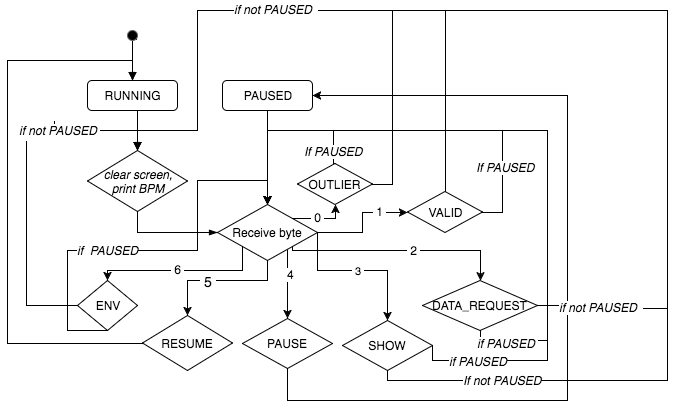
\includegraphics{ino.png}

\newpage

C Program

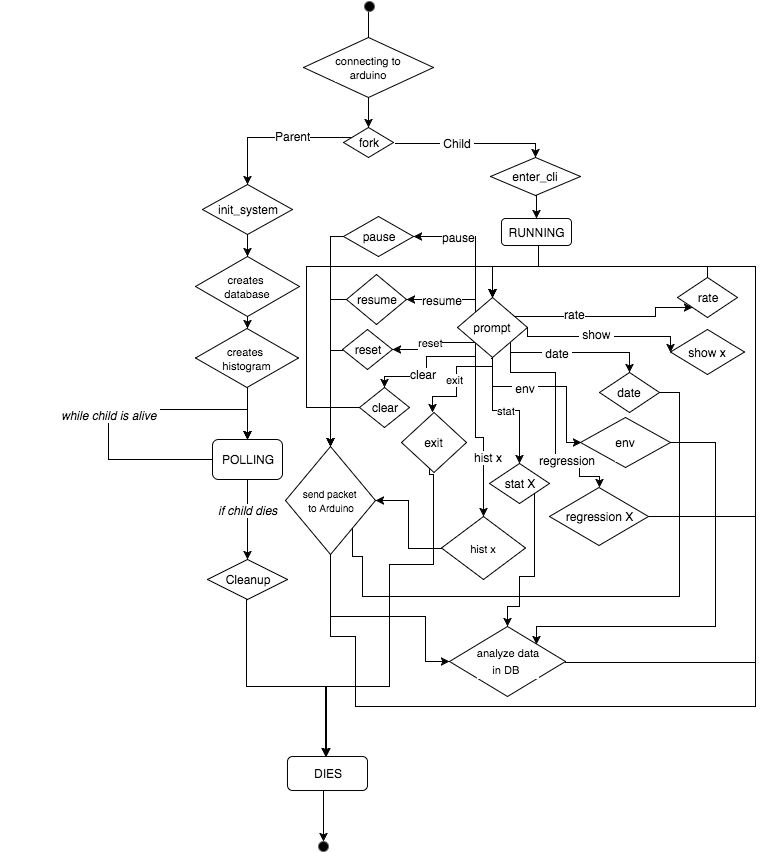
\includegraphics{c.png}

\section{Additional Specifications}\label{additional-specifications}

\begin{itemize}
\tightlist
\item
  Outlier Detection

  \begin{itemize}
  \tightlist
  \item
    To detect ouliers, we first wait until the program has collected at
    least 15 data points for the current bucket. Within the first 15
    data points, a reading is only an outlier if the heart rate is
    outside the range 30-200. After the first 15 data points, points
    that are not within two standard deviations of the mean are
    considered outliers for the current bucket.
  \end{itemize}
\item
  Time Synchronization

  \begin{itemize}
  \tightlist
  \item
    Upon starting, the Arduino waits for the C code to send the time
    data. Once it has recieved the data over Serial, it forwards it to
    the RTC, setting the time. Once this exchange has taken place, the
    programs each enter their respective state machines.
  \end{itemize}
\item
  Building Sensor Reading Pairs

  \begin{itemize}
  \tightlist
  \item
    For regression analysis, we build sensor reading pairs using SQL.
    The SQL query
    \texttt{SELECT\ bpm\_avg.avg\_bpm\ AS\ bpm\_reading,\ env\_avg.avg\_env\ AS\ env\_reading\ FROM\ (SELECT\ AVG(bpm)\ AS\ avg\_bpm,\ minute\_num\ FROM\ BPM\ GROUP\ BY\ minute\_num)\ as\ bpm\_avg,\ (SELECT\ AVG(env)\ AS\ avg\_env,\ minute\_num\ FROM\ ENV\ GROUP\ BY\ minute\_num)\ as\ env\_avg\ WHERE\ bpm\_avg.minute\_num\ =\ env\_avg.minute\_num\ AND\ bpm\_avg.minute\_num\ \textgreater{}=\ \%d\ AND\ bpm\_avg.minute\_num\ \textless{}\ \%d;}
    successfully pairs readings by minute numbers within a particular
    bucket. We then use these pairs to calculate the regression.
  \end{itemize}
\item
  Avoiding Concurrency Issues

  \begin{itemize}
  \tightlist
  \item
    To avoid having concurrency issues between the CLI process and the
    data polling process, we have the data polling process store its
    last bpm and env reading into mmap'd memory. When the \texttt{rate}
    or \texttt{env} command are called from the command line, it simply
    accesses the corresponding value in that mmap'd memory instead of
    having to make a request to the Arduino, as that may cause
    concurrency issues.
  \end{itemize}
\end{itemize}

\end{document}
